\RequirePackage{amsmath,amssymb}

\documentclass[runningheads, a4paper]{llncs}
\usepackage{lineno}
\usepackage{booktabs}
\usepackage{listings}
\usepackage{tcolorbox}
\usepackage{tikz}
\usepackage{tkz-graph}
\usepackage{stmaryrd}
\usepackage{wrapfig}

\usetikzlibrary{shapes.geometric, arrows}

\tikzstyle{startstop} = [rectangle, rounded corners, minimum width=3cm, minimum height=1cm,text centered, draw=black, fill=red!30]
\tikzstyle{process} = [rectangle, minimum width=3cm, text width=0.3*\columnwidth, minimum height=1cm, text centered, draw=black, fill=orange!30]
\tikzstyle{decision} = [diamond, minimum width=3cm, minimum height=1cm, text centered, draw=black, fill=green!30]
\tikzstyle{arrow} = [thick,->,>=stealth]


\renewcommand\linenumberfont{\normalfont\tiny\sffamily\color{red}}

\lstset{literate={~} {$\sim$}{1}, language=haskell, deletekeywords={abs},basicstyle=\ttfamily}

\newcommand{\expr}[1]{(#1)} % Expression quasiquote
\newcommand{\rarr}{\rightarrow}
\newcommand{\Rarr}{\Rightarrow}
\newcommand{\rewrites}{\Longrightarrow}

\newcommand{\exprt}[1]{\expr{\ttt{#1}}}
\newcommand{\tdots}{\ttt{...}}
\newcommand{\exprdots}{\expr{\tdots}}

\newcommand{\typeeq}{\raise.17ex\hbox{$\scriptstyle\mathtt{\sim}$}\,\;}

\newcommand{\ttt}{\texttt}

\newenvironment{todo}
  {\ifthenelse{\isundefined{\showtodos}}{\comment}{\begin{tcolorbox}
    \textbf{TODO}:}}
  {\ifthenelse{\isundefined{\showtodos}}{\endcomment}{\end{tcolorbox}}
  }
\newenvironment{todont}
               {\comment}
               {\endcomment}
\AtBeginDocument{%
  \providecommand\BibTeX{{%
    \normalfont B\kern-0.5em{\scshape i\kern-0.25em b}\kern-0.8em\TeX}}}

\begin{document}

\title{On Adding Pattern Matching to Haskell-based
  Deeply Embedded Domain Specific Languages}

\titlerunning{On Adding Pattern Matching to Haskell-based EDSLs}

\author{David Young\inst{1} \and Mark Grebe\inst{2} \and Andy Gill\inst{1}}
\institute{University of Kansas\\\email{$\{$d063y800,andygill$\}$@ku.edu} \and University of Central Missouri\\\email{grebe@ucmo.edu}}



\maketitle

\begin{abstract}
% Say what problem is
  Capturing control flow is the Achilles heel of Haskell-based
  deeply embedded domain specific languages.
  Rather than use
  the builtin control flow mechanisms, artificial control flow combinators
  are used instead.
% Say why it is an interesting problem
  However, capturing traditional control flow in a deeply embedded domain specific language
  would support the writing of programs in a natural style by allowing the programmer to use the
  constructs that are already builtin to the base language, such as pattern
  matching and recursion.
% Say what our solution achieves
  In this paper, we expand the capabilities of
  Haskell-based deep embeddings with a compiler extension
  for reifying conditionals and pattern matching.
% Here is why the world will be a better place
  With this new support, the subset of Haskell that we use for expressing
  deeply embedded domain specific languages can be cleaner, Haskell-idiomatic,
  and more declarative in nature.

\end{abstract}

\section{Introduction}

Embedded domain specific languages (EDSLs) have long been an effective
technique for constructing reusable tools for working in a variety of
different problem domains. Haskell is a language which is particularly
well-suited to EDSLs due to its lazy evaluation, first-class functions and
lexical closures.
%
Despite these advantages Haskell provides for creating EDSLs, there are a few
constructs for which representations have proven illusive. One prominent example
is that of a \ttt{case} expression. Pattern matching is a convenient way to
implement control flow structures and to inspect data structures, so it is
frequently a desirable feature for many EDSLs.
%
Additionally, lambdas can also be difficult to implement in EDSLs. A major reason
for this is that control flow constructs which are typically \textit{outside} the EDSL,
such as pattern matching and tail recursion, can make it challenging to ``look inside''
the lambda. When these control structures are reified within the EDSL, it is
easier to also reify lambdas using the dummy argument technique described in~\cite{Elliott:03:CompileDSEL-JFP}.


\begin{todo}
  Make it more clear how to integrate these concepts with other EDSLs. Maybe we should
  add a feature to the underlying implementation that allows an existing EDSL to be
  ``enriched'' with pattern matching support.
\end{todo}

The following contributions are made by this paper:

\begin{itemize}
  \item A representation of pattern matching in a Haskell EDSL (Section~\ref{sec:PatRep})
  \item A representation of lambdas (Section~\ref{sec:LamRep}) in the EDSL, utilizing
  the fact that both pattern matching and tail recursion are already captured in
  the EDSL.
  \item A GHC Core plugin which transforms a subset of standard Haskell code
  into this EDSL for pattern matching, extended with tail recursion,
  lambdas and primitive operations (Section~\ref{sec:CorePlugin})
  \item An implementation of an interpreter for a reference semantics of the EDSL (Section~\ref{sec:StdSemantics}).
\end{itemize}

Readers who are primarily interested only in the encoding of pattern matching itself can direct
most of their attention to Sections~\ref{sec:ADTRep},~\ref{sec:PatRep} and~\ref{sec:StdSemantics}. Most of the technical aspects of
the transformation performed by the Core plugin are described in Section~\ref{sec:CorePlugin}.

\subsection{Motivation}

A major benefit of the Haskell language is that it is frequently possible to derive
a Haskell implementation from a specification, either partially or fully.  This
technique is used extensively, for example, in \cite{Bird:2010:Pearls} and
\cite{Gibbons:2002:Calc}.  Recent examples of this technique include the work in
\cite{Elliott-2018-ad-icfp} as well as the work in
\cite{Elliott2019-convolution-extended}.  When it is not possible to fully
derive an implementation from a specification, it is often easier to check a
Haskell implementation against a specification than it is in many imperative
languages due, in part, to the management of side effects in Haskell. This is
more difficult to do using an imperative language such as C, as they provide no
restrictions on where side effects can occur.

Haskell EDSLs that support powerful language features like pattern matching
allow these advantages to be brought to problem domains where it is currently
either difficult or impossible to use a language that has these benefits.
However, there is no support for capturing pattern matching builtin to the Haskell
language itself. As a result, EDSLs which capture pattern matching must do so
via a plugin in a Haskell compiler such as GHC. For each such EDSL, this mechanism
has needed to be reimplemented each time. Additionally, the task of implementing this
is difficult and error-prone. In this paper, we descibe a \textit{reusable}
framework for capturing pattern matching, as well as lambdas and tail recursion.

\subsection{Overview}
\label{sec:Overview}

In this EDSL, the type representing values in the expression language is \ttt{E
t} and there are two basic functions which translate values to and from this
expression language with the following type signatures (omitting type class
constraints for the moment):

\begin{lstlisting}
rep :: a -> E a
abs :: E a -> a
\end{lstlisting}

\noindent Additionally, the following functions mark the parts of the code which the Core
plugin will target:

\begin{lstlisting}
internalize :: E a -> a
externalize :: a -> E a
\end{lstlisting}

\noindent The \ttt{E} type is the type of expressions in the EDSL.  In this paper, the
data constructors of this type will be described incrementally as they
are needed.

\subsection{Translation Example}

In the example below, the Core plugin transforms \verb|example| into
\verb|example'|. Note that \verb|example'| is an EDSL expression which is then
used by the EDSL interpreter function \verb|abs| to produce the final result,
\verb|example''|:

\begin{lstlisting}[deletekeywords={Ord}]
x :: Either Char Int
x = Left 'a'

example :: E Int
example =
  externalize (case x of Left c -> ord c; Right i -> i)

example' :: E Int
example' = CaseExp (LeftExp (CharLit 'a'))
  (SumMatchExp
    (OneProdMatch (Lam 1 (Ord (Var 1))))
    (OneSumMatch (OneProdMatch (Lam 2 (Var 2)))))

example'' :: Int
example'' = abs example'
\end{lstlisting}

\section{Representing Algebraic Datatypes}
\label{sec:ADTRep}

Briefly, an algebraic type \ttt{T} with an automatically generated \ttt{ERep}
instance is given a representation in terms of \ttt{Either}, \ttt{(,)}, \ttt{()}
and \ttt{Void}.  This ``standardized'' type representation is given by \ttt{ERepTy
T}. \ttt{ERepTy} is a type family associated to the type class \ttt{ERep}. This
type will be called the \textit{canonical type} of \ttt{T}.

Only the ``outermost'' type will be deconstructed into these fundamental building
blocks, and further deconstruction can take place on these pieces later on. For
example, consider this type:

\begin{lstlisting}
data ComplexPair =
  ComplexPair (Complex Double) (Complex Double)
  deriving (Generic, Show)

instance ERep ComplexPair
\end{lstlisting}

\noindent Note the instance definition is automatically generated from the \ttt{Generic}
instance.

Given this code, the following type equality holds:
\\

\ttt{ERepTy ComplexPair \typeeq (Complex Double, Complex Double)}
\\
\noindent Here is an example that demonstrates why this is more useful than if it \textit{fully} deconstructed
each type into \ttt{Either}, \ttt{(,)} and \ttt{()}:

\begin{lstlisting}
sumComplexPair :: ComplexPair -> Complex Double
sumComplexPair p =
  internalize (externalize
    (case p of ComplexPair a b -> a + b))
\end{lstlisting}

\noindent If \ttt{ERepTy ComplexPair} were fully deconstructed into \ttt{((Double, Double),
(Double, Double))}, we would need a \ttt{Num} instance for \ttt{(Double,
Double)}.  What we really want is to use the fact that a \ttt{Num} instance
already exists for \ttt{Complex Double}. This is exactly what preserving this
type information allows us to do. We can later use this preserved type
information in backends, through the corresponding \ttt{Typeable} instances (for
instance, to provide special support for arithmetic on complex numbers).

It is important to note that we are still able to further deconstruct this type
with further pattern matches, since \ttt{ERepTy (Complex Double) \typeeq (Double, Double)}:

\begin{lstlisting}
realSum :: ComplexPair -> Double
realSum p =
  internalize (externalize
    (case p of
      ComplexPair a b ->
        case a of
          a_real :+ _ ->
            case b of
              b_real :+ _ ->
                a_real + b_real))
\end{lstlisting}

\noindent The above pattern matches could also be written as a single nested pattern
match. Both forms compile down to the same Core representation.

An additional benefit of this is that recursive types require no special handling. For
example, consider:

\begin{lstlisting}
data IntList = Nil | Cons Int IntList
  deriving (Generic, Show)

instance ERep IntList
\end{lstlisting}

\noindent Note that \ttt{ERepTy IntList \typeeq Either () (Int, IntList)}. If \ttt{ERepTy}
attempted to ``fully deconstruct'' \ttt{IntList}, it would send the compiler
into an infinite loop.

This allows us to implement functions on such recursive types:

\begin{lstlisting}
isEmpty :: IntList -> Bool
isEmpty t =
  internalize (externalize
    (case t of
      Nil -> True
      Cons x xs -> False))

intListSum :: (Int, IntList) -> Int
intListSum p =
  internalize (externalize
    (case p of (acc, t) -> case t of
       Nil -> acc
       Cons x xs ->
         intListSum
           (x+acc, xs)))
\end{lstlisting}

\subsection{The Three Major Type-Level Pieces}

There are three interconnected foundational parts: \ttt{E}, \ttt{ERep} and
\ttt{ERepTy}. \ttt{E} is the deep embedding of the EDSL (a GADT~\cite{Vytiniotis:2006:Simple} that encodes
expressions in the DSL language). \ttt{ERep} is a type class which represents
all Haskell types which can be represented in the DSL. \ttt{ERepTy} is a type
family associated to the \ttt{ERep} type class, which represents a ``canonical form''
of the given type. This canonical form can be immediately constructed in the EDSL.
Canonical form types crucially include \ttt{Either} and \ttt{(,)}, which
allow all combinations of basic sum types and product types to be encoded, in the
manner described at the beginning of Section~\ref{sec:ADTRep}.

With GHC Generics, any data type \ttt{T} with a \ttt{Generic} instance has a
corresponding \ttt{Rep T} type, which gives a generic representation of \ttt{T}.
Conversion between values of this type and values of the original type \ttt{T} is
given by the functions \ttt{to} and \ttt{from}. The generic representation \ttt{Rep T}
can be traversed by functions which operate solely on the structure of the data type.
This generic representation contains additional metadata which we do not need.
However, we can automatically generate a \ttt{ERep} instance for any type which
has a \ttt{Generic} instance.

As \ttt{Generic} instances are automatically generated, this provides a simple mechanism
to automaticly generate \ttt{ERep} instances.


This information is brought into the \ttt{E} type via the constructor
\ttt{ConstructRep}. The \ttt{E} also contains constructors representing \ttt{Either}
and \ttt{(,)} values:

\begin{lstlisting}
data E t where
  ...
  ConstructRep :: (Typeable a, ERep a) =>
    E (ERepTy a) -> E a
  LeftExp :: E a -> E (Either a b)
  RightExp :: E b -> E (Either a b)
  PairExp :: E a -> E b -> E (a, b)
  ...
\end{lstlisting}

\noindent \ttt{ERep} and \ttt{ERepTy} provide an interface for transferring values between the EDSL
expression language and the source Haskell language:

\begin{lstlisting}
class Typeable t => ERep t where
  type ERepTy t
  construct :: t -> E (ERepTy t)
  rep :: t -> E t
  default rep :: (ERep (ERepTy t)) => t -> E t
  rep x = ConstructRep (construct x)
  unrep' :: ERepTy t -> t
  rep' :: t -> ERepTy t
\end{lstlisting}

\noindent The key algebraic instances mentioned before are as follows:

\begin{lstlisting}
instance (ERep a, ERep b) => ERep (Either a b) where
  type ERepTy (Either a b) = Either a b
  construct (Left x)  = LeftExp (rep x)
  construct (Right y) = RightExp (rep y)
  rep (Left x)  = LeftExp (rep x)
  rep (Right y) = RightExp (rep y)
  unrep' = id
  rep'   = id

instance (ERep a, ERep b) => ERep (a, b) where
  type ERepTy (a, b) = (a, b)
  construct (x, y) = PairExp (rep x) (rep y)
  rep (x, y) = PairExp (rep x) (rep y)
  unrep' = id
  rep'   = id
\end{lstlisting}



\section{Representing pattern matching}
\label{sec:PatRep}

Within the \ttt{E} expression language, a pattern match is represented by the
\ttt{CaseExp} constructor:
\begin{lstlisting}
data E t where
  ...
  CaseExp :: (ERep t, ERepTy (ERepTy t) ~ ERepTy t) =>
    E t -> E (SumMatch (ERepTy t) r) -> E r
  ...
\end{lstlisting}

\noindent The equality constraint ensures that a canonical type is its own canonical type.

The above code block is a slight simplification of the actual implementation,
which has an additional type variable which is used at an ``intermediate'' point.
The expanded form is in place to simplify the Core transformation.

The type \ttt{SumMatch} is defined as

\begin{lstlisting}
newtype SumMatch a b =
  MkSumMatch { runSumMatch :: a -> b }
\end{lstlisting}

\noindent For the moment, we will primarily use this type as a type tag and ignore
the values it can take on.

A value of type \ttt{E (SumMatch a b)} represents a computation within the EDSL
which destructures a value of type \ttt{E a} and produces a value of type \ttt{E b}.
Therefore, \ttt{E (SumMatch (ERepTy t) r)} represents a computation which destructures
a value of type \ttt{E (ERepTy t)} and produces a value of type \ttt{E r}.



\subsection{\ttt{E (SumMatch a b)}}

The overall structure of a \ttt{E (SumMatch a b)} value is a (heterogeneous)
list of \ttt{E (ProdMatch x b)} values.  Each item of this list corresponds
exactly to one branch in the original \ttt{case} match.

The following constructors generate \ttt{SumMatch}-tagged values in the
expression language:

\begin{lstlisting}
data E t where
  ...
  SumMatchExp :: (ERep a, ERep b, ERepTy b ~ b) =>
    E (ProdMatch a r) -> E (SumMatch b r)
      -> E (SumMatch (Either a b) r)

  OneSumMatch ::
    (ERep a, ERep b, ERepTy a ~ a) =>
      E (ProdMatch a b) -> E (SumMatch a b)
  EmptyMatch :: (ERep b) => E (SumMatch Void b)
\end{lstlisting}

\noindent Note the \ttt{ERepTy a \typeeq a} constraints. This constraint ensures that the type
\ttt{a} is already in canonical form (that is, consists entirely of
\ttt{Either}, \ttt{(,)} and base types).

\subsection{\ttt{E (ProdMatch s t)}}

\ttt{E (ProdMatch s t)} is equivalent to a function from \ttt{s} to
\ttt{t} in the expression language where \ttt{s} is a (potentially
nested) pair type. For example, \ttt{E (ProdMatch (a, (b, c)) r)} is
equivalent to \ttt{E (a -> E (b -> E (c -> E r)))}.

\begin{lstlisting}
data E t where
  ...
  ProdMatchExp :: (ERep a, ERep b) =>
    E (a -> ProdMatch b r) -> E (ProdMatch (a, b) r)

  NullaryMatch :: (ERep a) =>
    E r -> E (ProdMatch a r)

  OneProdMatch :: (ERep a) =>
    E (a -> b) -> E (ProdMatch a b)
  ...
\end{lstlisting}

The \ttt{ProdMatch} type is defined similarly to the \ttt{SumMatch} type and is
similiarly used primarily as a type tag:

\begin{lstlisting}
newtype ProdMatch a b =
  MkProdMatch { runProdMatch :: a -> b }
\end{lstlisting}


\subsection{An aside on \ttt{ProdMatch} and \ttt{SumMatch} values}
\label{sec:MatchAside}

Though \ttt{ProdMatch} and \ttt{SumMatch} are used throughout this EDSL as type
tags, they do have values and they are not trivial values. The reason for this
is that it connects the encoded pattern matches (values from the \ttt{E}) type
to their semantics. A value of type \ttt{E (SumMatch a b)} is an expression
which takes in a value of type \ttt{a} (embedded within the expression
language), internally performs some pattern matching, and produces a value of
type \ttt{b} (again, embedded within the expression language). This is exactly
the semantics of a function from \ttt{a} to \ttt{b}. Likewise for \ttt{ProdMatch a b}.

Recall the previously mentioned function

\begin{lstlisting}
abs :: E a -> a
\end{lstlisting}

\noindent Now consider at the type of \ttt{abs} when it is specialized to take
\ttt{E (SumMatch a b)} values:

\begin{lstlisting}
abs :: E (SumMatch a b) -> SumMatch a b
\end{lstlisting}

\noindent If we postcompose with \ttt{runSumMatch}, we get:

\begin{lstlisting}
runSumMatch . abs    :: E (SumMatch a b) -> (a -> b)
\end{lstlisting}

\noindent The \ttt{SumMatch a b} value which \ttt{abs} returns is exactly the function
which pattern matches according to its input value. Likewise for \ttt{ProdMatch a b} values.

\section{Representing tail recursion}
Tail recursion is given a direct-style representation using a simple sum type,
using the technique described in~\cite{Grebe:2017:RSD:3136040.3136048}.

Consider a tail recursive function of the type \ttt{f :: a -> b}. Each recursive
call can be seen as a simple ``update'' of the values of the arguments, since
these calls are all in tail position. This is why tail recursive functions
can be easily compiled to simple loops or conditional jumps.

We can take advantage of this view by transforming a tail recursive function
\ttt{f :: a -> b} into a function \ttt{f' :: a -> Iter b a}. \ttt{Iter b a} is a
type which can either correspond to an argument ``update'' (in the sense mentioned
previously) or a final result. This type is implemented as a sum of the types
\ttt{a} and \ttt{b}. Recursive calls are transformed to \ttt{Step} applications
and non-recursive branches are wrapped in \ttt{Done} applications.

\begin{lstlisting}
data Iter a b = Step b | Done a
  deriving (Functor, Generic)
\end{lstlisting}

\noindent To use the new \ttt{f'} function, we repeatedly call it until it gives a
\ttt{Done} value. If it gives a \ttt{Step} value, we pass the the value wrapped
in the \ttt{Step} back into \ttt{f'} and continue.

The function \ttt{runIter} provides the reference semantics for executing such a
function representing a tail recursive function:

\begin{lstlisting}
runIter :: (ERep a, ERep b)
  => (a -> Iter b a) -> (a -> b)
runIter f = go
  where go x = case f x of
          Done r  -> r
          Step x' -> go x'
\end{lstlisting}


\noindent This technique can be contrasted with the more traditional trampolining
technique for implementing tail recursion. Conventional trampolining uses a
sum type of the result type and a thunk with the code necessary to continue
execution.~\cite{Ganz:99:Trampolined}

In the technique presented here, we do not need to allocate thunks or closures.
We do not need to use higher-order functions for this representation, other than \ttt{runIter} itself.

In the \ttt{E} type of our DSL, this form of tail recursion representation is
given a deep embedding by the following constructors:

\begin{lstlisting}
data E t where
  ...
  StepExp :: E b -> E (Iter a b)
  DoneExp :: E a -> E (Iter a b)
  TailRec :: (ERep a, ERep b) =>
    E (b -> Iter a b) -> E (b -> a)
  ...
\end{lstlisting}

\noindent The process of transforming a tail recursive function in the DSL to a 
representation which could be passed into a backend and used
to generate a traditional iterative loop goes as follows.

Starting with the tail recursive function  \ttt{isEven}:

\begin{lstlisting}
isEven :: Int -> Bool
isEven x =
  internalize (externalize (
    case x == 0 of
      True -> True
      False ->
        case x == 1 of
          True -> False
          False -> isEven (x - 2)))
\end{lstlisting}


\noindent We first transform this to use the \verb|Iter| type. The lambda is brought
inside of the \ttt{internalize (externalize ...)} call and wrapped in a call to
\ttt{runIter}. This inner expression is then eta expanded. Finally, each \verb|case|
branch which does not contain a recursive call is wrapped in a \verb|Done| and
every recursive call is transformed into an application of the \verb|Step| constructor.

In the following code, \verb|eta| is a fresh variable.

\begin{lstlisting}
isEven' :: Int -> Bool
isEven' =
  internalize (externalize
    (\ eta ->
      runIter (\ x -> case x == 0 of
                        True -> Done True
                        False -> case x == 1 of
                            True -> Done False
                            False -> Step (x - 2))
              eta))
\end{lstlisting}

\noindent After this initial tail recursion transformation, the rest of the plugin brings this
result into the expression language. \verb|TailRec| is substituted for \verb|runIter|,
\verb|DoneExp| is substituted for \verb|Done| and \verb|StepExp| is substituted for \verb|Step|.
Next, the pattern matching transformation occurs, producing the final result:


\begin{lstlisting}
isEven'' :: Int -> Bool
isEven'' =
  internalize (
    (Lam (Var 1)
      (App (TailRec (Lam (Var 2)
             (IfThenElseExp (Equal (Var 2) (rep 0))
               (DoneExp TrueExp)
               (IfThenElseExp (Equal (Var 1) (rep 1))
                 (DoneExp FalseExp)
                 (StepExp (Sub (Var 2) (rep 2)))))))
           (Var 1))))
\end{lstlisting}

\section{Representing lambdas}
\label{sec:LamRep}

This representation of pattern matching depends on the ability to bring
function values into the expression language. This is accomplished
with the following constructors:

\begin{lstlisting}
data E t where
  ...
  Lam :: (ERep a, Typeable a) =>
    Name a -> E b -> E (a -> b)
  Var :: (Typeable a) => Name a -> E a
\end{lstlisting}

\noindent The \ttt{Typeable} constraints are necessary to lookup correctly typed
values in the variable binding environment later on.

The \ttt{Name t} type represents a lambda variable identifier together with its
type \ttt{t} (Note that the \ttt{ScopedTypeVariables} extension is enabled):

\begin{lstlisting}
newtype Name a = Name Int deriving (Eq, Show)

namesEq :: forall a b.  (Typeable a, Typeable b) =>
  Name a -> Name b -> Maybe (a :~: b)
namesEq (Name n) (Name n') =
  case eqT :: Maybe (a :~: b) of
    Just Refl
      | n == n'   -> Just Refl
      | otherwise -> Nothing
    Nothing       -> Nothing
\end{lstlisting}

\noindent In the Core transformation, each lambda is given a \ttt{Name} with a globally
unique \ttt{Int}, sidestepping any name capture issues.

The following datatypes are used to represent a variable binding environment
of typed names to expression language values:

\begin{lstlisting}
data EnvMapping where
  (:=>) :: forall a. Typeable a =>
    Name a -> E a -> EnvMapping
\end{lstlisting}

\noindent This type encodes a single variable binding, with values of the form
\ttt{n :=> v}, where \ttt{n} is a typed name and \ttt{v} is the value it is bound to.

These bindings are grouped together in the \ttt{Env} type:
% \newpage
\begin{lstlisting}
newtype Env = Env [EnvMapping]

emptyEnv :: Env
emptyEnv = Env []

extendEnv :: Env -> EnvMapping -> Env
extendEnv (Env maps) m = Env (m:maps)

envLookup :: Typeable a => Env -> Name a -> Maybe (E a)
envLookup (Env maps) = go maps
  where
    go []                = Nothing
    go ((n' :=> e):rest) =
      case namesEq n n' of
        Just Refl -> Just e
        Nothing   -> go rest
\end{lstlisting}


\section{Recovering reference semantics for pattern matches}
\label{sec:StdSemantics}

The reference semantics for the EDSL is given by \ttt{abs}. Two helper
functions, \ttt{sumMatchAbs} and \ttt{prodMatchAbs}, are used to provide
the reference semantics for matches on sum types and matches on product
types, respectively. These helper functions are based on the mechanism
described in Section~\ref{sec:MatchAside}.

\begin{lstlisting}
abs :: forall t. E t -> t
abs = absEnv emptyEnv

sumMatchAbs :: (ERepTy (ERepTy s) ~ ERepTy s, ERep s)
  => Env -> E (SumMatch (ERepTy s) t) -> s -> t
...
prodMatchAbs :: (ERep s) =>
  Env -> E (ProdMatch s t) -> s -> t
...
\end{lstlisting}

\noindent Recall that the internal representations of \verb|SumMatch a b| and \verb|ProdMatch a b|
are functions of type \verb|a -> b|. These types are unwrapped by the functions

\begin{lstlisting}
runSumMatch :: SumMatch a b -> (a -> b)
runProdMatch :: ProdMatch a b -> (a -> b)
\end{lstlisting}

\noindent Given this, the \verb|ProdMatchExp| case of the \verb|prodMatchAbs| function can be
implemented as follows:

\begin{lstlisting}
prodMatchAbs env (ProdMatchExp f) = \ pair ->
  case pair of (x, y) ->
    runProdMatch (absEnv env f x) y
\end{lstlisting}

\noindent See Appendix A for implementation details of \ttt{absEnv}.



\section{Core Plugin}
\label{sec:CorePlugin}

The Core plugin translates marked expressions. Expressions are marked by
the \ttt{externalize} function:

\begin{lstlisting}
externalize :: a -> E a
\end{lstlisting}

\noindent For example, \ttt{externalize x} marks the expression \ttt{x}.  If an expression
already has an EDSL type (a type of the form \ttt{E a} for some \ttt{a}), then
the marking procedure ignores it and does not wrap it with \ttt{externalize}
(see $M$ in Figure~\ref{fig:Rewrites}).

These \verb|externalize| marks are pushed through the input program, starting at
the outermost level. The plugin repeatedly runs over each newly marked node in
the abstract syntax tree, applying the appropriate rewrite rules as it goes.
This process pushes the marks through the program until it reaches a base case
that has no proper subexpressions, such as a character literal.

The plugin's control flow is described in Figure~\ref{fig:CorePlugin}. When control
flow reaches a node, the rewrite rules listed in parentheses are performed. These rewrite
rule names correspond to the rules given in Figure~\ref{fig:Rewrites}.
%
In Figure~\ref{fig:Rewrites},
$\varepsilon$ represents an empty term (in the context of the term rewriting system used in that Figure). Calls
to \ttt{unrep :: E a -> a} are only used internally and will not exist in
the final result of the transformation.

\begin{figure}
  \centering
  \resizebox{0.8\columnwidth}{8.2cm}{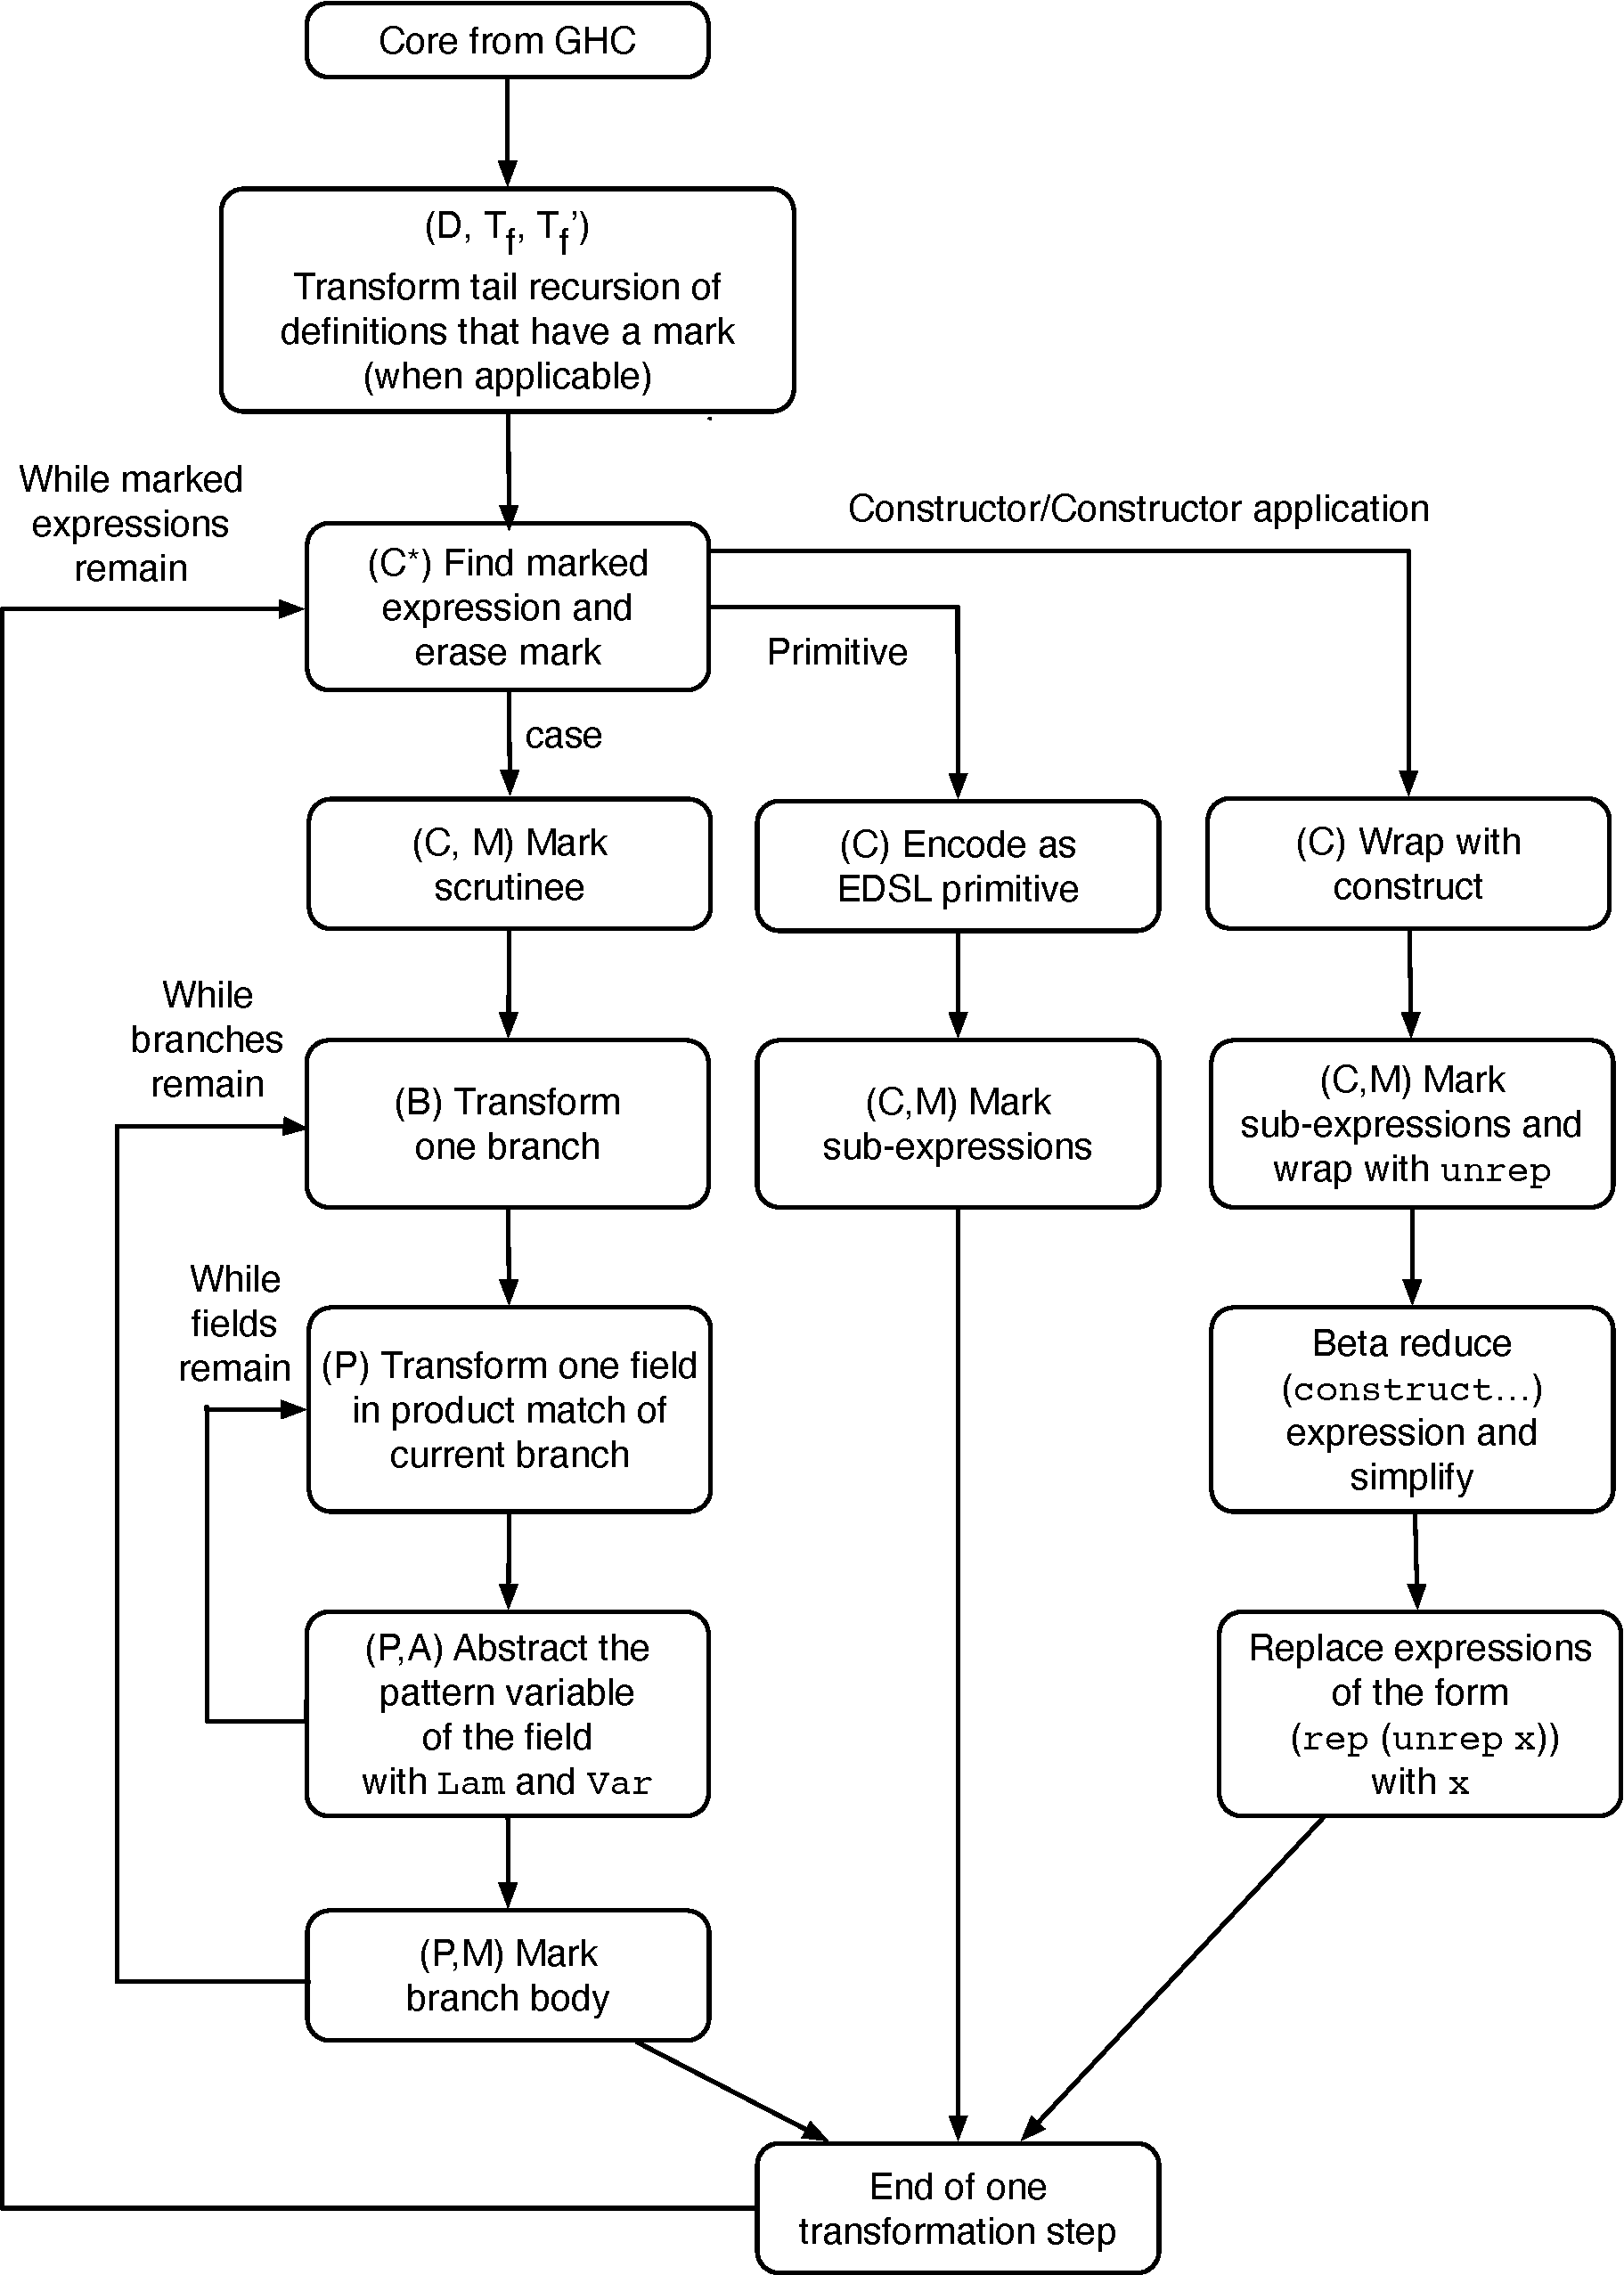
\includegraphics{Diagrams/Flowchart.pdf}}
   \caption{Control Flow of the Core Plugin}
   \label{fig:CorePlugin}
\end{figure}%

\pagebreak
Note that:
\begin{itemize}
  \item The tail recursion transformation given by $D$, $T'_{\ttt{f}}$ and $T_{\ttt{f}}$ is completely independent of the \ttt{E} type and the transformations associated to the \ttt{E} type. As a result, the tail recursion transformation can be used on its own.

  \item The total number of marks introduced is upper bounded by the number of
subexpressions in the original Core given to the transformation by GHC and each
full transformation step (that is, $C$) eliminates one mark. Therefore, the
transformation will terminate.
\end{itemize}

\begin{figure}
  \centering
\resizebox{1\linewidth}{!}{
  \begin{minipage}{\linewidth}
\begin{align*}
  &D\expr{\ttt{f x = internalize (externalize (case s of \{ ... \}))}}\\
      &\quad\rewrites I(D(\ttt{f x = externalize (case s of \{ ... \})}))\\
  &D\expr{\ttt{f x = externalize (case s of \{ ... \})}}\\
      &\quad\rewrites \begin{cases}
        \ttt{f = $C^{*}\expr{\ttt{externalize ($\lambda \eta \rarr$ runIter ($\lambda \ttt{x} \rarr \ttt{case s of \{ $T'_{\ttt{f}}\exprdots$}$ \}) $\eta$)}}$} & \text{\parbox{2.4cm}{if \ttt{f} occurs free in \ttt{\{ ... \}}, where $\eta$ is a fresh name}}\\
        \\
        \ttt{f x = $C^{*}\expr{\ttt{externalize (case s of \{ ... \})}}$} & \text{otherwise}
      \end{cases}\\
  &\\
  &I\expr{\ttt{f x = externalize e}} \rewrites \ttt{f x = internalize (externalize e)}\\
  &I\expr{\ttt{f = externalize e}} \rewrites \ttt{f = internalize (externalize e)}\\
  &T'_{\ttt{f}}\expr{\ttt{K x0 ...$_U$ xN $\rarr$ case s of \{ ...$_V$ \}; ...$_W$}}\\
    &\quad\rewrites
        \ttt{K x0 ...$_U$ xN $\rarr$ $T_{\ttt{f}}\expr{\ttt{case s of \{ ...$_V$ \}}}$; $T'_{\ttt{f}}\expr{\ttt{ ...$_W$ }}$}\\
  &T'_{\ttt{f}}\expr{\ttt{K x0 ...$_U$ xN $\rarr$ body0; ...$_V$ }}\\
    &\quad\rewrites
      \begin{cases}
        \ttt{K x0 ...$_U$ xN $\rarr$ body0}[\ttt{f} \mapsto \ttt{Step}]\ttt{; }T'_{\ttt{f}}\expr{\ttt{ ...$_V$ }} & \text{if \ttt{f} occurs free in \ttt{body0}}\\
        \ttt{K x0 ...$_U$ xN $\rarr$ Done body0; $T'_{\ttt{f}}\expr{\ttt{ ...$_V$ }}$} & \text{otherwise}
      \end{cases}\\
  &T'_{\ttt{f}}\expr{\varepsilon} \rewrites \varepsilon\\
  &T_{\ttt{f}}\expr{\ttt{case s of \{ ... \}}}\\
    &\quad\rewrites
      \begin{cases}
        \ttt{case s of \{ $T'_{\ttt{f}}\expr{\ttt{ ... }}$ \}} & \text{if \ttt{f} occurs free in \ttt{\{ ... \}}}\\
        \ttt{Done (case s of \{ ... \})} & \text{otherwise}
      \end{cases}\\
  &C^{*}\expr{\ttt{x}} \rewrites
    \begin{cases}
      \ttt{x} & \text{if \ttt{x} has no subexpressions marked with \ttt{externalize}}\\
      C^{*}\expr{C\expr{\ttt{y}}} & \text{if \ttt{externalize y} is the first marked subexpression of \ttt{x}}\\
    \end{cases}\\
  &C\expr{\ttt{runIter f x}} \rewrites \ttt{App (TailRec $M\expr{\ttt{f}}$) $M\expr{\ttt{x}}$}\\
  &C\expr{\ttt{x + y}} \rewrites \ttt{Add $M\expr{\ttt{x}}$ $M\expr{\ttt{y}}$}\\
  &C\expr{\ttt{case scrutinee of \{ ... \}}} \rewrites \ttt{CaseExp $M\expr{\ttt{scrutinee}}$ } B\expr{\ttt{ ... }}\\
  &C\expr{\ttt{$\lambda$x $\rarr$ body}} \rewrites A\expr{\lambda \ttt{x} \rarr \ttt{body}}\\
  &C\expr{\ttt{K x0 ... xN }}\\
    &\quad\rewrites \ttt{construct (K (unrep $M\expr{\ttt{x0}}$) ... (unrep $M\expr{\ttt{xN}}$))}\;\;\;\;\text{(Where \ttt{K} is a constructor)}\\
  &C\expr{\ttt{f x}} \rewrites \ttt{App $M\expr{f}$ $M\expr{x}$}\\
  &B\expr{\ttt{K x0 ...$_U$ xN $\rarr$ body0; ...$_V$}} \rewrites \ttt{SumMatchExp }P\expr{\ttt{x0 ...$_U$ xN $\rarr$ body0}}\; B\expr{\ttt{ ...$_V$ }}\\
  &B\expr{\ttt{K x0 ... xN $\rarr$ body}} \rewrites \ttt{OneSumMatchExp }P\expr{\ttt{x0 ... xN $\rarr$ body}}\\
  &B\expr{\ttt{$\varepsilon$}} \rewrites \ttt{EmptyMatch}\\
  &P\expr{\ttt{x0 x1 ... xN $\rarr$ body}} \rewrites \ttt{ProdMatchExp }A\expr{\ttt{$\lambda$ x0 $\rarr$ $P\expr{\ttt{x1 ... xN $\rarr$ body}}$}}\\
  &P\expr{\ttt{x $\rarr$ body}} \rewrites \ttt{OneProdMatchExp }A\expr{\ttt{$\lambda$ x $\rarr$ body}}\\
  &P\expr{\ttt{ $\rarr$ body}} \rewrites \ttt{NullaryMatch $M\expr{\ttt{body}}$}\\
  &A\expr{\ttt{$\lambda$(x :: a) $\rarr$ body}} \rewrites \ttt{Lam (Name @a uniq) $M\expr{\ttt{body$[\ttt{x} \mapsto \ttt{unrep (Var @a uniq)}]$}}$}\\
  &\text{\;\;\;\;\;(where \ttt{uniq} is a globally unique identifier)}\\
  &M\expr{\ttt{unrep x}} \rewrites \ttt{x}\\
  &M\expr{\ttt{x :: a}} \rewrites
    \begin{cases}
      \ttt{externalize x} & \text{if}\; \nexists t, a\; \typeeq E\; t\\
      \ttt{x} & \text{if}\; \exists t, a\; \typeeq E\; t
    \end{cases}
\end{align*}
  \end{minipage}
}%

\caption{Rewrite rules}
\label{fig:Rewrites}

\end{figure}

\section{Related Work}


The basis of deep embeddings in functional languages is well understood.
\cite{Elliott:03:CompileDSEL-JFP} explains the basic idea, and \cite{Gill:2014:DSLSynth}
gives an accessable and more recent account of the area.

A similar EDSL-oriented representation of pattern matching is given in
~\cite[Section~3.3]{Atkey:09:Unembedding}. In that paper, patterns were given their own
representation which allows for compound patterns. This is useful in the context
of that work, as the programmer works directly with these patterns.

In the present paper, however, the representation is generated automatically by
a compiler plugin. As a result of GHC's desugared Core (which does not have
compound patterns), there is no need to directly express compound patterns at
the representation-level.

There is other recent work using deep embeddings in functional languages for 
system development.  One example is the Ivory language \cite{Elliott2015-Ivory} 
which provides a deeply embedded DSL for use in programming high assurance
systems,  However, its syntax is typical of a deep EDSL and requires additional
keywords and structures above idiomatic Haskell. 

The Feldspar project~\cite{Axelsson:10:Feldspar,Svenningsson:13:Combining}
is a Haskell embedding of a monadic interface
that targets C, and focuses on high-performance.  Both Feldspar and our work
mix deep and shallow language constructs ~\cite{Persson:11:MonadicDSL,Svenningsson:13:Compositional,Sculthorpe:13:ConstrainedMonad}.

Svenningsson and Axelsson~\cite{Svenningsson:13:Combining}
explored combining deep and shallow embedding.  They used
a deep embedding as a low level language, then extended
the deep embedding with a shallow embedding written on top
of it. Haskell type classes were used to minimize the effort of adding
new features to the language.

Yin-Yang~\cite{Jovanovic:2014} provides a framework for DSL
embedding in Scala which uses Scala macros to provide the 
translation from a shallow to deep embedding.  Yin-Yang
goes beyond the translation by also providing autogeneration
of the deep DSL from the shallow DSL.  The focus of
Yin-Yang is in generalizing the shallow to deep transformations,
and does not include recursive transformations.

Forge~\cite{Sujeeth:2013} is a Scala based meta-EDSL framework
which can generate both shallow and deep embeddings from
a single EDSL specification.  Embeddings generated by Forge
use abstract \verb|Rep| types, analogous to our EDSL's 
\verb|E| types.  Their shallow embedding is generated
as a pure Scala library, while the deeply embedded version
is generated as an EDSL using the Delite~\cite{Sujeeth:2014}
framework.

Elliott developed GHC plugins~\cite{github:lambda-ccc}\cite{github:reification-rules}
for compiling Haskell to hardware~\cite{github:Elliott:Talk:2015},
using worker-wrapper style transformations~\cite{Gill:09:WW}
equivalent to the \verb|abs| and
\verb|rep| transformations described in Section~\ref{sec:Overview}. These plugins were later generalized to enable additional interpretations~\cite{Elliott:2017}.

\section{Conclusion}

\begin{todo}
Should some of this go into the introduction?
\end{todo}

In this paper, a representation of pattern matching was given in the form of a
GADT called \verb|E|. A GHC plugin is then used to transform code written in a
subset of Haskell consisting of algebraic data types, pattern matching, tail
recursion and lambdas into values of this GADT. A backend can then use these
\verb|E a| values to interpret the Haskell code, compile it or otherwise
manipulate it.

Additionally, a uniform representation of algebraic data types in terms of
\verb|(,)|, \verb|Either| and \verb|()|, called \verb|ERepTy|, was outlined for
use in the previously mentioned pattern matching representation. This
representation of ADTs is determined entirely by the structure of a type,
allowing the pattern matching mechanism to act on the structure of values.


\begin{todo}
Should we have a diagram somewhere in the paper to show how these pieces all fit together?
\end{todo}

\newpage
\bibliographystyle{splncs04}
\bibliography{paper}


\end{document}
\endinput
